% Provenance (never printed): old premiere S material on the oceanic lithosphere
% (ophiolite-type layering, peridotite and gabbro, partial melting by decompression
% at the ridge, hydrothermalism, cooling and subsidence of the lithosphere with
% age); see sources/book2/PROVENANCE.md. Melting from figdata/grade-11/
% ridge_melting.py (adiabat and Hirschmann solidus), depth against age from
% depth_age.py (ETOPO1 and the Seton 2020 age grid). Partial melting is re-founded
% in Year 2 (mantle-melting); fault is Book 1's (g7), normal fault is defined here.
\chapter{洋脊与大洋岩石圈}\label{ch:g11:ocean-ridges}

1977 年 2 月，一台照相机雪橇被拖到 2500 米深处，掠过东太平洋的加拉帕戈斯
裂谷上方，拍下了洋脊上光秃秃的黑色熔岩，
一帧接一帧。随后温度计记录到水温有小幅上升，
照片上熔岩表面覆满了
数百只白色蛤蜊。几天后，载人潜水器\emph{Alvin}号
载着两位地质学家下潜到该地点：温暖而闪烁的海水正从
熔岩裂缝中涌出，周围生活着前臂那么长的蛤蜊，
贻贝和白色蟹；后来一次下潜中还见到了顶部发红的管虫。没有人
料到那里会有生命，所以船上没有生物学家。本章将解释
地质学家发现了什么：洋底在洋脊处如何形成，
为什么那里很热，以及它远离洋脊后会发生什么变化。
% ledger: whoi:alvin-1977

\begin{recall}
在洋脊处，新的洋底不断生成并向两侧移开，因此
其年龄随离开轴线的距离而增大；洋脊构成一个约
\qty{65000}{km}长的系统，慢速洋脊处为裂谷，
快速洋脊处为光滑的脊顶（见\cref{ch:g11:drift-to-spreading}）。
板块在洋脊两侧相互分离，每年约几厘米，东太平洋海隆上
的分离快于大西洋中脊（见\cref{ch:g11:plate-motions}）。
\omterm{def:g11:lithosphere-asthenosphere:lithosphere}{岩石圈}是坚硬的外壳，其下的\omterm{def:g11:lithosphere-asthenosphere:lithosphere}{软流圈}会流动；\omterm{def:g11:lithosphere-asthenosphere:lithosphere}{软流圈}的温度
每千米仅升高约 \qty{0.45}{\celsius}，
而地幔岩石的熔化温度随深度增加而升高
（见\cref{ch:g11:lithosphere-asthenosphere}）。岩浆是地表之下的熔融岩石，
玄武岩是熔岩冷却时形成的暗色岩石，断层则是岩石沿其发生过位移的
断裂面（第 1 册，六、七年级）。
\end{recall}
% ledger: noaa:ridge, katsura10:adiabat, hirschmann:solidus

\section{大洋岩石圈}

地表大陆上少见的两种岩石，构成了大部分
\omterm{def:g11:ocean-ridges:oceanic-lithosphere}{大洋岩石圈}。

\begin{definition}[橄榄岩]\label{def:g11:ocean-ridges:peridotite}
\emph{橄榄岩}\index{橄榄岩}是一种暗色粗粒岩石，
主要由矿物橄榄石构成，并含有一些辉石。通常呈绿色，
质地致密。人们认为地幔的大部分由橄榄岩构成。
\end{definition}

\begin{definition}[辉长岩]\label{def:g11:ocean-ridges:gabbro}
\emph{辉长岩}\index{辉长岩}是一种暗色粗粒火成岩，
主要由斜长石和辉石构成，其化学成分与
玄武岩相同，但它在地下深处缓慢结晶，使晶体
有时间长大。它是大洋深部地壳中最丰富的岩石。
\end{definition}
% ledger: geo:peridotite, geo:gabbro

此处提到的矿物橄榄石、辉石和长石，
详见\cref{ch:g11:minerals}。

\begin{omfigure}
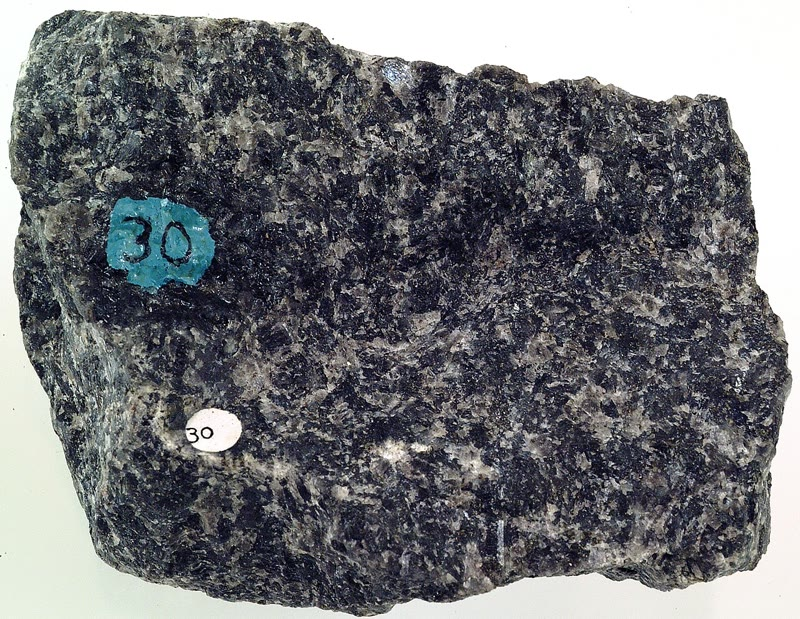
\includegraphics[height=4.2cm]{images/book2/g11-geodil-gabbro.jpg}\hspace{0.03\linewidth}%
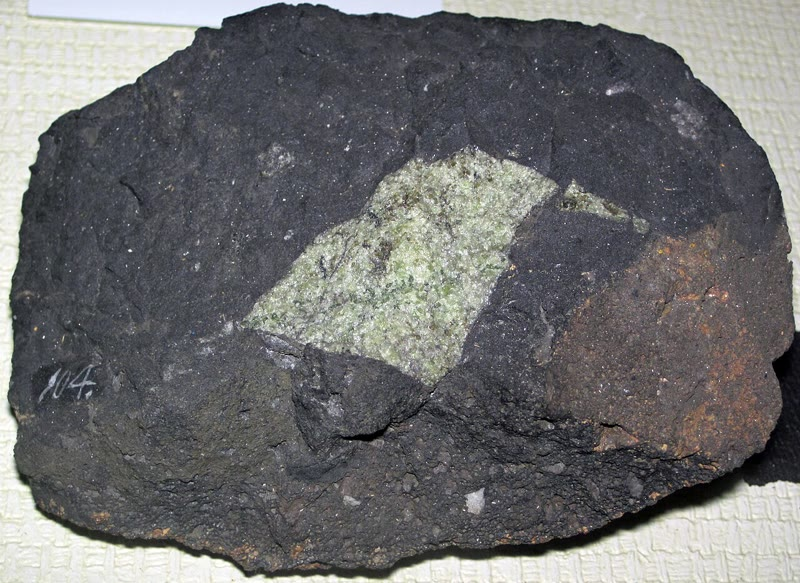
\includegraphics[height=4.2cm]{images/book2/g11-stjohn-peridotite.jpg}

{\small 左：\omterm{def:g11:ocean-ridges:gabbro}{辉长岩}，直径 \qty{9}{cm}，暗色辉石与浅色
长石晶体肉眼清晰可见；照片：Darla Sondrol（CC0）。
右：一块来自地幔的绿色\omterm{def:g11:ocean-ridges:peridotite}{橄榄岩}，被裹挟在
亚利桑那州一座火山的黑色玄武岩熔岩之中；照片：James St.~John（CC~BY~2.0）。}
\end{omfigure}
% ledger: photo:g11-gabbro, photo:g11-peridotite

\begin{definition}[洋壳；大洋岩石圈]\label{def:g11:ocean-ridges:oceanic-lithosphere}
\emph{洋壳}\index{洋壳}是海底的地壳，
厚约 \qty{7}{km}，由玄武岩和\omterm{def:g11:ocean-ridges:gabbro}{辉长岩}构成，形成于洋脊处。
\emph{大洋岩石圈}\index{大洋岩石圈}是洋壳
与其下最上部地幔中坚硬的\omterm{def:g11:ocean-ridges:peridotite}{橄榄岩}共同组成。
\end{definition}

全球各大洋的地震测量表明，\omterm{def:g11:ocean-ridges:oceanic-lithosphere}{洋壳}的平均
厚度为 \qty{7.1}{km}，上下浮动约 \qty{0.8}{km}，不计
断裂带和热点区域。其分\omterm{def:g10:layered-ocean:stratification}{层结}构由深钻以及
被推上大陆的古老洋底岩片所证实。2005 年，一艘钻探船
完成了一个深 \qty{1507}{m} 的钻孔，钻入 1500 万年的
东太平洋\omterm{def:g11:ocean-ridges:oceanic-lithosphere}{洋壳}，这是首次从熔岩经岩墙直达
\omterm{def:g11:ocean-ridges:gabbro}{辉长岩}的钻探：
% ledger: white92:crust, iodp1256:section, geo:peridotite

\begin{itemize}
  \item 顶部是一层薄薄的\emph{沉积物}，洋脊
        轴部没有，在较老的洋底上更厚；
  \item 超过 \qty{800}{m} 的\emph{玄武岩熔岩}，在海底
        以席状和\emph{枕状熔岩}的形式喷发，即圆管状和团块状
        熔岩，表面为玻璃质外壳；
  \item \emph{席状岩墙}，本孔中厚 \qty{346}{m}：数百条
        竖直的玄武岩板，每一块都是岩浆上升至喷发时所经裂缝
        的凝固遗迹，并排排列，如同书页一样；
  \item \emph{\omterm{def:g11:ocean-ridges:gabbro}{辉长岩}}，在海底以下 \qty{1407}{m} 处钻遇，岩浆
        在岩墙之下缓慢结晶，直至\omterm{def:g11:seismic-structure:moho}{莫霍面}；
  \item \omterm{def:g11:seismic-structure:moho}{莫霍面}之下为地幔的\emph{\omterm{def:g11:ocean-ridges:peridotite}{橄榄岩}}。
\end{itemize}
% ledger: iodp1256:section, geo:basalt-ridges, geo:gabbro

\begin{omfigure}
\begin{tikzpicture}[x=1cm, y=-0.55cm, font=\footnotesize]
% to scale in depth: lavas 0.8 km, dykes 0.35 km (iodp1256:section), crust 7.1 km (white92:crust)
  \fill[omLithAlluv] (0,-0.25) rectangle (2.4,0);
  \fill[lith basalt] (0,0) rectangle (2.4,0.8);
  \fill[omLithBasalt!60] (0,0.8) rectangle (2.4,1.15);
  \foreach \x in {0.15,0.35,...,2.3} \draw[black!55, line width=0.3pt] (\x,0.8) -- (\x,1.15);
  \fill[lith gabbro] (0,1.15) rectangle (2.4,7.1);
  \fill[lith peridotite] (0,7.1) rectangle (2.4,9.0);
  \draw (0,-0.25) rectangle (2.4,9.0);
  \draw[line width=0.9pt] (0,7.1) -- (2.4,7.1);
  \foreach \d in {0,2,4,6,8} {\draw (-0.1,\d) -- (0,\d); \node[anchor=east] at (-0.1,\d) {\d};}
  \node[rotate=90, anchor=south] at (-0.75,4.5) {海底以下深度（\unit{km}）};
  \draw[black!60] (2.4,-0.13) -- (2.7,-1.0) -- (2.85,-1.0);
  \node[anchor=west] at (2.85,-1.0) {沉积物};
  \draw[black!60] (2.4,0.4) -- (2.7,0.25) -- (2.85,0.25);
  \node[anchor=west] at (2.85,0.25) {熔岩：枕状熔岩与席状流};
  \draw[black!60] (2.4,0.98) -- (2.7,1.6) -- (2.85,1.6);
  \node[anchor=west] at (2.85,1.6) {席状岩墙};
  \node[anchor=west] at (2.55,4.1) {辉长岩};
  \node[anchor=west] at (2.55,7.1) {莫霍面};
  \node[anchor=west] at (2.55,8.05) {地幔橄榄岩};
  \draw[decorate, decoration={brace, amplitude=5pt}] (7.9,0) -- (7.9,7.1)
    node[midway, right=7pt, align=left] {洋壳 \\约 \qty{7}{km}};
\end{tikzpicture}

{\small \omterm{def:g11:ocean-ridges:oceanic-lithosphere}{洋壳}各层按深度比例绘制。熔岩与岩墙的
厚度取自东太平洋的深钻孔；\omterm{def:g11:ocean-ridges:oceanic-lithosphere}{洋壳}总厚度
取自地震测量的平均值。沉积物覆盖层
随海底年龄增大而增厚。}
\end{omfigure}
% ledger: iodp1256:section, white92:crust

\begin{omfigure}
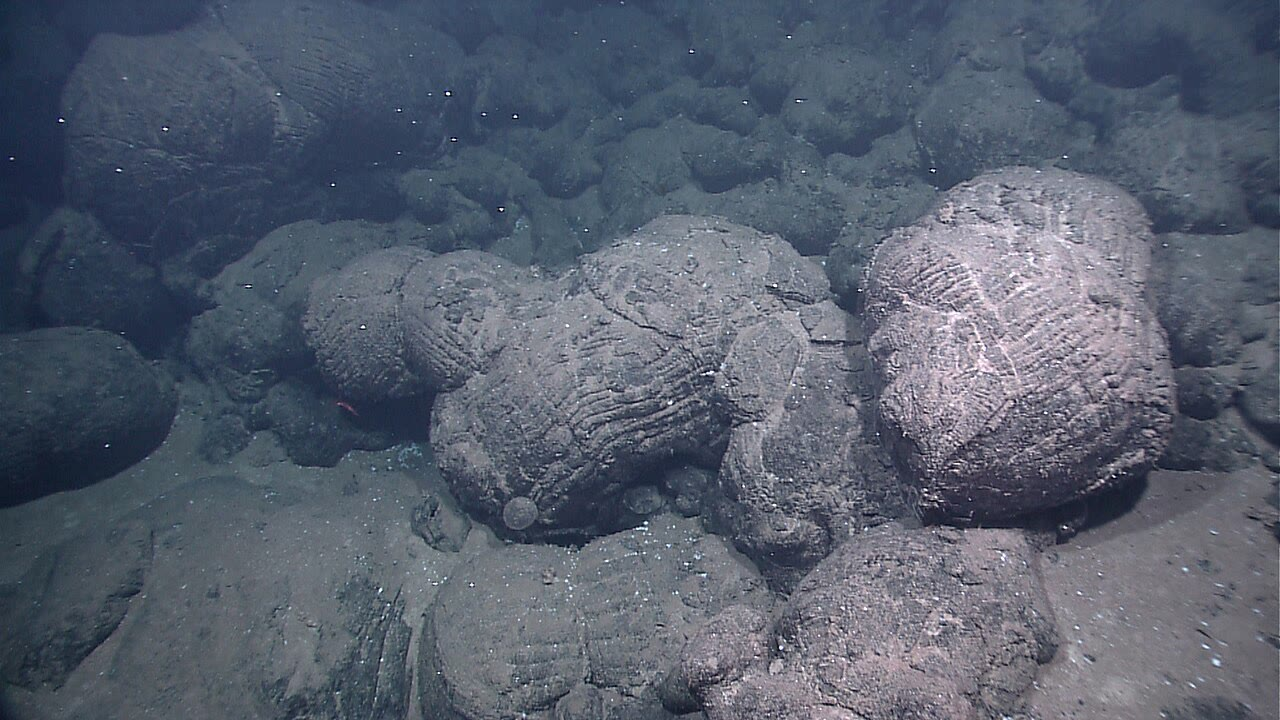
\includegraphics[width=0.8\linewidth]{images/book2/g11-noaa-pillow-lava.jpg}

{\small 加拉帕戈斯裂谷的枕状熔岩，位于约 2500 米深处，
2011 年由遥控潜水器拍摄。每个枕状体都是一段舌状熔岩，
它一接触冷海水便从外部开始凝固。
照片：NOAA Okeanos Explorer Program（公有领域）。}
\end{omfigure}
% ledger: photo:g11-pillow-lava, whoi:alvin-1977 (depth of the rift floor)

\section{无需加热的熔化}

洋脊之下的地幔与其他地方一样，是固态的\omterm{def:g11:ocean-ridges:peridotite}{橄榄岩}。然而
\qty{7}{km} 厚的玄武岩与\omterm{def:g11:ocean-ridges:gabbro}{辉长岩}，即凝固的熔融岩石，都出自它。
熔体从何而来？

\begin{definition}[部分熔融；减压熔融]\label{def:g11:ocean-ridges:partial-melting}
\emph{部分熔融}\index{部分熔融}指岩石中只有一部分发生熔化，
即其中某些矿物或其组分发生熔化，而
其余部分仍保持固态。
\emph{减压熔融}\index{减压熔融}指上升的岩石受压逐渐减小，
在不加热的情况下发生的部分熔融。
\end{definition}

两板块相互分离时，\omterm{def:g11:lithosphere-asthenosphere:lithosphere}{软流圈}在洋脊之下上涌，
以填补空隙。上涌过快，岩石几乎来不及散热，因此
上升时温度每千米仅下降约 \qty{0.45}{\celsius}。
其熔化温度取决于压强，下降要快得多，约为
每千米 \qty{3.9}{\celsius}（在 \qty{50}{km} 深处）。
上升的岩石在某一深度达到其熔化温度并开始熔化，
尽管并未额外加热。
% ledger: katsura10:adiabat, hirschmann:solidus, white92:crust; computed in
% figdata/grade-11/ridge_melting.py (solidus_slope_50km 3.89)

\begin{method}[上升的地幔在何处熔化？]\label{met:g11:ocean-ridges:melting}
\begin{enumerate}
  \item 写出上升岩石在各深度的温度：即其
        位温（即岩石升至地表时的温度）
        再加上深度每千米增加的 \qty{0.45}{\celsius}。
  \item 根据各深度的压强，写出岩石在该深度的
        熔化温度。
  \item 求两者相等的深度。在更深处，岩石为固态；
        在较浅处，岩石\omterm{def:g11:ocean-ridges:partial-melting}{部分熔融}。
\end{enumerate}
\end{method}

\begin{omfigure}
\begin{tikzpicture}
\begin{axis}[omrecord, omdepth, width=0.72\linewidth, height=6.4cm, xmin=1100, xmax=1700, ymin=0, ymax=150,
  xlabel={温度（\unit{\celsius}）}, ylabel={深度（\unit{km}）},
  xticklabel style={/pgf/number format/set thousands separator={}}, clip=true]
% computed in figdata/grade-11/ridge_melting.py; ledger: katsura10:adiabat, hirschmann:solidus, data:prem
\addplot[omProp, line width=1.0pt] table[x=solidus, y=z] {figdata/out/grade-11-ridge_melting-curves.dat};
\addplot[omDef, line width=1.0pt] table[x=ad1300, y=z] {figdata/out/grade-11-ridge_melting-curves.dat};
\addplot[omDef, densely dashed, line width=0.9pt] table[x=ad1400, y=z] {figdata/out/grade-11-ridge_melting-curves.dat};
\addplot[only marks, mark=*, mark size=1.8pt, black] coordinates {(1324.3,54.1) (1438.3,85.0)};
\node[font=\scriptsize, anchor=east, align=right] at (axis cs:1316,62) {熔化始于，\\深 \qty{54}{km}};
\node[font=\scriptsize, anchor=east] at (axis cs:1432,89) {\qty{85}{km}};
\node[font=\scriptsize, text=omProp, anchor=west, align=left] at (axis cs:1560,40) {熔化 \\温度};
\node[font=\scriptsize, text=omDef, anchor=east, align=right] at (axis cs:1318,128) {上升的地幔，\\$T_p = \qty{1300}{\celsius}$};
\node[font=\scriptsize, text=omDef, anchor=west, align=left] at (axis cs:1476,140) {$T_p = \qty{1400}{\celsius}$};
\end{axis}
\end{tikzpicture}

{\small 洋脊之下上升的地幔岩石温度（蓝色）及其
熔化温度（橙色）随深度的变化。位温为
\qty{1300}{\celsius} 的岩石在 \qty{54}{km} 深处开始熔化；
位温高 \qty{100}{\celsius} 的岩石（虚线）在 \qty{85}{km} 深处即已开始熔化。
而干\omterm{def:g11:ocean-ridges:peridotite}{橄榄岩}的熔化温度取自实验（Hirschmann, 2000）。}
\end{omfigure}
% values: onset_1300_km 54.1, onset_1400_km 85.0, t_onset_1300 1324 (ridge_melting.py)

\begin{example}[熔化开始的深度]\label{ex:g11:ocean-ridges:onset}
若地幔位温为 \qty{1300}{\celsius}，上升的岩石
升至 \qty{54}{km} 深处时温度为 $1300 + 0.45 \times 54 \approx \qty{1324}{\celsius}$，
恰好等于该深度的熔化温度：熔化在约 \qty{54}{km} 深处开始。
在此深度以上，岩石随上升继续熔化。
\end{example}

只有一小部分\omterm{def:g11:ocean-ridges:peridotite}{橄榄岩}熔化，熔体并非\omterm{def:g11:ocean-ridges:peridotite}{橄榄岩}，
而是玄武岩。玄武岩熔体从整个熔融区汇聚，该区域
从起始深度一直延伸至地壳底部；玄武岩熔体密度小于周围固态岩石，
因此上升至洋脊轴部。那里，部分岩浆喷出
成为熔岩，部分在上升时穿过的裂隙中凝固为岩墙，另一部分
在深处缓慢结晶为\omterm{def:g11:ocean-ridges:gabbro}{辉长岩}。留下的固态\omterm{def:g11:ocean-ridges:peridotite}{橄榄岩}
因玄武岩被抽离而亏损，成为\omterm{def:g11:ocean-ridges:oceanic-lithosphere}{大洋岩石圈}的地幔部分。
% ledger: asimow01:morb, geo:basalt-ridges, white92:crust

洋脊穿过地幔较热的区域，例如热点附近时，熔化
开始得更深，熔融的岩柱更长，生成的玄武岩也更多：于是
地壳厚约 \qty{10}{km}，而非 7 千米。相反，在极慢速的
洋脊之下，上升的地幔有时间散热，熔化较少，
并形成异常薄的地壳。
% ledger: white92:crust

\begin{omfigure}
\begin{tikzpicture}[font=\footnotesize]
  % schematic section across a ridge axis, not to scale
  \fill[omSea!45] (-6,0) rectangle (6,1.2);
  \fill[lith basalt] (-6,0) -- (-0.25,0) -- (-0.25,-0.35) -- (-6,-0.6) -- cycle;
  \fill[lith basalt] (6,0) -- (0.25,0) -- (0.25,-0.35) -- (6,-0.6) -- cycle;
  \fill[lith gabbro] (-6,-0.6) -- (-0.25,-0.35) -- (-0.25,-1.4) -- (-6,-1.6) -- cycle;
  \fill[lith gabbro] (6,-0.6) -- (0.25,-0.35) -- (0.25,-1.4) -- (6,-1.6) -- cycle;
  \fill[lith basalt] (-0.3,0) rectangle (0.3,-0.35);
  \fill[lith gabbro] (-0.3,-0.35) rectangle (0.3,-1.45);
  \fill[omProp!70] (-0.8,-0.75) .. controls (-0.4,-0.55) and (0.4,-0.55) .. (0.8,-0.75)
     .. controls (0.4,-0.95) and (-0.4,-0.95) .. (-0.8,-0.75);
  \fill[omProp!70] (-0.12,0) rectangle (0.12,-0.62);
  \fill[lith peridotite] (-6,-1.6) -- (-0.25,-1.4) -- (0.25,-1.4) -- (6,-1.6) -- (6,-5) -- (-6,-5) -- cycle;
  % melting region
  \fill[omProp!35] (-3.2,-1.5) -- (0,-4.0) -- (3.2,-1.5) -- cycle;
  \node[align=center] at (0,-2.95) {熔融区};
  % isotherms deepening away from the axis
  \draw[omDef!70!black, densely dashed] (-6,-2.6) .. controls (-2.5,-2.0) and (-1,-1.1) .. (0,-1.0) .. controls (1,-1.1) and (2.5,-2.0) .. (6,-2.6);
  \draw[omDef!70!black, densely dashed] (-6,-4.2) .. controls (-3,-3.6) and (-1.2,-2.0) .. (0,-1.9) .. controls (1.2,-2.0) and (3,-3.6) .. (6,-4.2);
  \node[text=omDef!70!black, anchor=west] at (6.05,-2.6) {\qty{800}{\celsius}};
  \node[text=omDef!70!black, anchor=west] at (6.05,-4.2) {\qty{1200}{\celsius}};
  % flow arrows
  \draw[-{Stealth[length=5pt]}, line width=0.9pt] (0,-4.9) -- (0,-4.2);
  \draw[-{Stealth[length=5pt]}, line width=0.9pt] (-1.2,-4.8) .. controls (-1.0,-3.8) and (-2.2,-3.2) .. (-3.6,-3.2);
  \draw[-{Stealth[length=5pt]}, line width=0.9pt] (1.2,-4.8) .. controls (1.0,-3.8) and (2.2,-3.2) .. (3.6,-3.2);
  \draw[-{Stealth[length=5pt]}, line width=1.1pt] (-2,0.6) -- (-4,0.6);
  \draw[-{Stealth[length=5pt]}, line width=1.1pt] (2,0.6) -- (4,0.6);
  \node[anchor=south] at (-3,0.65) {板块};
  \node[anchor=south] at (3,0.65) {板块};
  \node[anchor=west] at (1.0,-0.8) {岩浆透镜体};
  \node[anchor=east] at (-6.05,-0.3) {熔岩};
  \node[anchor=east] at (-6.05,-1.1) {辉长岩};
  \node[anchor=east] at (-6.05,-3.3) {地幔};
  \node[anchor=north] at (0,-5.05) {地幔上升并熔化};
\end{tikzpicture}

{\small 沿洋脊轴线的剖面（示意图，未按比例绘制）。地幔
在轴线下方上升并\omterm{def:g11:ocean-ridges:partial-melting}{部分熔融}；熔融物在轴线下方聚集成岩浆透镜体
并形成地壳，地壳随板块被带向
两侧。等温线（虚线）在轴线处靠近地表，
离轴线越远越深，\omterm{def:g11:lithosphere-asthenosphere:lithosphere}{岩石圈}
随冷却而增厚。}
\end{omfigure}

\section{快速洋脊与慢速洋脊}

洋脊张开的速度差别很大。根据
\cref{ch:g11:plate-motions}中的旋转极计算，南纬 \ang{30} 处的东太平洋海隆每年张开
\qty{14.6}{cm}，同纬度的大西洋中脊每年张开
\qty{3.3}{cm}。两者轴部的形态并不相同。
% ledger: nnr56:poles (computed in plate_velocities.py: epr30s_speed 145.8, atl30s_speed 32.7)

慢速洋脊的轴部是一条山谷，深 1 至 \qty{2}{km}，宽 20
至 \qty{30}{km}。到达轴部的岩浆太少，无法
持续填补空隙：冷而脆的\omterm{def:g11:lithosphere-asthenosphere:lithosphere}{岩石圈}被拉开，并沿
断层断裂。

\begin{definition}[正断层]\label{def:g11:ocean-ridges:normal-fault}
称\emph{正断层}\index{正断层}为一种倾斜断层，沿该断层
断层面上方的岩块相对下方岩块向下移动。
正断层形成于地壳被拉伸的地方。
\end{definition}

慢速洋脊的山谷是夹在\omterm{def:g11:ocean-ridges:normal-fault}{正断层}之间下落的岩块，
两侧\omterm{def:g11:ocean-ridges:normal-fault}{正断层}相向，几乎都朝轴部倾斜。此类
在\omterm{def:g11:ocean-ridges:normal-fault}{正断层}之间下落的岩块称为\emph{地堑}。
% ledger: buck05:valley, usgs:normal-fault

快速洋脊处，岩浆到达得足够频繁，足以填补空隙。轴部是
一个平缓光滑的高地，位于其下的岩浆透镜体之上。
% ledger: buck05:valley, noaa:ridge

\begin{omfigure}
\begin{tikzpicture}[font=\footnotesize, x=0.24cm, y=0.9cm]
  % slow ridge: axial valley between normal faults (not to scale, vertical exaggeration)
  \begin{scope}
    \fill[omSea!45] (-15,-0.7) rectangle (15,1.6);
    \fill[lith basalt] (-15,0.9) -- (-9,0.9) -- (-8.5,0.2) -- (-6,0.2) -- (-5.5,-0.6) -- (5.5,-0.6)
      -- (6,0.2) -- (8.5,0.2) -- (9,0.9) -- (15,0.9) -- (15,-2.2) -- (-15,-2.2) -- cycle;
    \draw[black!70] (-15,0.9) -- (-9,0.9) -- (-8.5,0.2) -- (-6,0.2) -- (-5.5,-0.6) -- (5.5,-0.6)
      -- (6,0.2) -- (8.5,0.2) -- (9,0.9) -- (15,0.9);
    \draw[fault] (-9,0.9) -- (-7.4,-2.2);
    \draw[fault] (-6,0.2) -- (-4.6,-2.2);
    \draw[fault] (9,0.9) -- (7.4,-2.2);
    \draw[fault] (6,0.2) -- (4.6,-2.2);
    % slip arrows on the hanging walls (the axis side of each fault): down along the fault
    \foreach \x/\y/\s in {-7.9/-0.5/1, -5.0/-1.3/1, 7.9/-0.5/-1, 5.0/-1.3/-1} {
      \draw[-{Stealth[length=3pt]}, omProp, line width=0.8pt] (\x+0.9*\s,\y+0.45) -- ++(0.3*\s,-0.6);
    }
    \draw[-{Stealth[length=5pt]}, line width=1pt] (-11,1.25) -- (-14,1.25);
    \draw[-{Stealth[length=5pt]}, line width=1pt] (11,1.25) -- (14,1.25);
    \node at (0,-0.25) {轴部山谷};
    \node[anchor=north, align=center] at (0,-2.25) {慢速洋脊：\\正断层之间的山谷};
  \end{scope}
  % fast ridge
  \begin{scope}[xshift=8.2cm]
    \fill[omSea!45] (-15,0) rectangle (15,1.6);
    \fill[lith basalt] (-15,0.3) .. controls (-6,0.4) and (-2,0.9) .. (0,0.95) .. controls (2,0.9) and (6,0.4) .. (15,0.3)
      -- (15,-2.2) -- (-15,-2.2) -- cycle;
    \fill[omProp!75] (-2.5,-0.9) .. controls (-1,-0.7) and (1,-0.7) .. (2.5,-0.9) .. controls (1,-1.1) and (-1,-1.1) .. (-2.5,-0.9);
    \draw[black!70] (-15,0.3) .. controls (-6,0.4) and (-2,0.9) .. (0,0.95) .. controls (2,0.9) and (6,0.4) .. (15,0.3);
    \node[anchor=north] at (0,-1.25) {岩浆透镜体};
    \draw[-{Stealth[length=5pt]}, line width=1pt] (-8,1.25) -- (-14,1.25);
    \draw[-{Stealth[length=5pt]}, line width=1pt] (8,1.25) -- (14,1.25);
    \node at (0,1.3) {轴部隆起};
    \node[anchor=north, align=center] at (0,-2.25) {快速洋脊：\\岩浆透镜体上方的平缓隆起};
  \end{scope}
\end{tikzpicture}

{\small 慢速洋脊与快速洋脊的剖面（示意图，未按比例绘制；
高度经过夸大）。左图：慢速洋脊的轴部山谷，深 1 至
\qty{2}{km}，夹在向轴部倾斜的\omterm{def:g11:ocean-ridges:normal-fault}{正断层}之间下落；
（橙色箭头：断层上方的岩块向下滑动）。右图：快速洋脊
在岩浆透镜体上方平缓隆起。}
\end{omfigure}
% ledger: buck05:valley

\begin{example}[慢速洋脊与快速洋脊]\label{ex:g11:ocean-ridges:rates}
在一百万年内，南纬 \ang{30} 处的东太平洋海隆生成
$\qty{14.6}{cm/\text{年}} \times 10^6\ \text{年} = \qty{146}{km}$ 的新洋底，
洋底，每侧 \qty{73}{km}；同一纬度的大西洋中脊
生成 \qty{33}{km} 的新洋底，每侧 \qty{16.5}{km}。东太平洋的深钻孔
所钻入的\omterm{def:g11:ocean-ridges:oceanic-lithosphere}{洋壳}，生成速率超过每年 \qty{20}{cm}，
属有记录以来扩张最快者之一。
\end{example}
% ledger: nnr56:poles (computed), iodp1256:section

\section{热液喷口}

轴部年轻的地壳温度很高，并被裂隙割裂。海水
便由此渗入。

\begin{definition}[热液循环；黑烟囱]\label{def:g11:ocean-ridges:hydrothermal}
称\emph{热液循环}\index{热液循环}为海水的流动，
海水沿炽热\omterm{def:g11:ocean-ridges:oceanic-lithosphere}{洋壳}中的裂隙向下流动，在那里被下方的岩浆加热，
并与岩石发生反应，再向上流回海底，
并从\emph{热液喷口}流出。
称\emph{黑烟囱}\index{黑烟囱}为一种喷口，从中喷出
溶有金属的高温热水；遇冷海水时，硫化铁与
其他矿物沉淀为黑色烟云，并在喷口周围
堆砌出一座烟囱。
\end{definition}
% ledger: whoi:vents

\omterm{def:g11:ocean-ridges:hydrothermal}{黑烟囱}中的热水通常约在
\qty{350}{\celsius}处离开烟囱，喷口水温可达 \qty{400}{\celsius}。它们不会沸腾，
因为上方有两千五百米深的海水压着。
烟囱可长高逾 \qty{10}{m}。喷口周围，细菌
从喷口水中的硫化氢获取能量，并养活管虫、
虾和贻贝；加拉帕戈斯裂谷的蛤类便以此为生。大多数
喷口位于洋中脊沿线。
% ledger: whoi:vents, whoi:alvin-1977

\begin{omfigure}
\begin{minipage}[c]{0.6\linewidth}\centering
\begin{tikzpicture}[font=\scriptsize, x=0.8cm, y=0.62cm]
  \fill[omSea!45] (0,0) rectangle (10,3);
  \fill[lith basalt] (0,0) rectangle (10,-4);
  \fill[omProp!70] (2,-4.6) .. controls (4,-4.0) and (6,-4.0) .. (8,-4.6) -- (8,-5) -- (2,-5) -- cycle;
  \node at (5,-4.7) {岩浆};
  \fill[black!75] (4.7,0) -- (4.85,1.6) -- (5.15,1.6) -- (5.3,0) -- cycle;
  \fill[black!45, opacity=0.8] (5,1.7) circle (0.35) (5.2,2.2) circle (0.45) (4.9,2.7) circle (0.4);
  \draw[-{Stealth[length=4pt]}, omDef, line width=0.9pt] (1,0) .. controls (1,-2.5) and (2.5,-3.6) .. (4.2,-3.5);
  \draw[-{Stealth[length=4pt]}, omDef, line width=0.9pt] (9,0) .. controls (9,-2.5) and (7.5,-3.6) .. (5.8,-3.5);
  \draw[-{Stealth[length=4pt]}, omProp, line width=1.1pt] (5,-3.3) -- (5,-0.1);
  \node[align=center, text=omDef!80!black] at (1.6,1.0) {冷海水 \\流入};
  \node[align=left, anchor=west] at (5.6,1.4) {黑烟囱，\\约 \qty{350}{\celsius}};
  \node[align=left, anchor=west, text=omProp!80!black, fill=white, fill opacity=0.85, text opacity=1, inner sep=1.5pt] at (5.3,-1.8) {受热，\\上升};
\end{tikzpicture}
\end{minipage}\hfill
\begin{minipage}[c]{0.3\linewidth}\centering
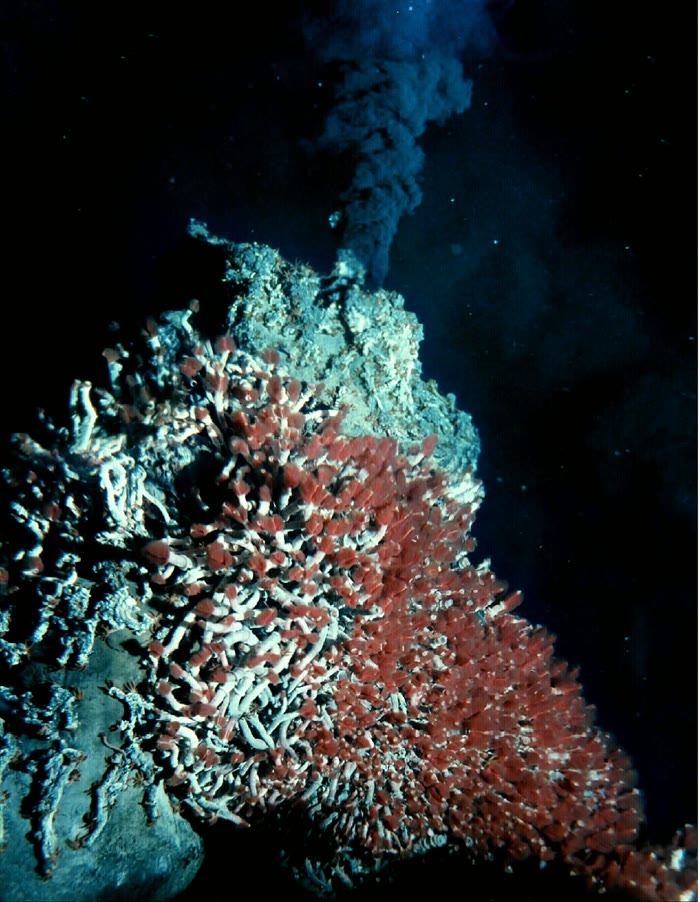
\includegraphics[width=\linewidth]{images/book2/g11-noaa-black-smoker.jpg}
\end{minipage}

{\small 左：洋脊轴部的\omterm{def:g11:ocean-ridges:hydrothermal}{热液循环}（示意图，未
按比例）。右：胡安·德富卡洋脊上的\omterm{def:g11:ocean-ridges:hydrothermal}{黑烟囱}，烟囱上覆满
红鳃管虫；照片由华盛顿大学与 NOAA 提供
（公有领域）。}
\end{omfigure}
% ledger: whoi:vents, photo:g11-black-smoker

\begin{history}[\emph{Alvin} 在加拉帕戈斯裂谷，1977 年]
该考察由美国国家科学基金会资助，于
1977 年 2 月 8 日乘科研船 \emph{Knorr} 出发。照相拖橇 ANGUS，
被拖至裂谷上方 \qty{2500}{m} 深处，记录到
水温升高；同一批照片显示，熔岩上有数百个白蛤
和褐色贻贝壳。在 \emph{Alvin} 号的第 713 次下潜中，
地质学家杰克·科利斯与蒂尔德·范安德尔发现，裂缝中涌出的水温为 \qty{8}{\celsius}，
随后升至 \qty{17}{\celsius}，而周围\omterm{def:g10:layered-ocean:thermocline}{深海}水温仅为
\qty{2}{\celsius}；白蛤最长达 \qty{30}{cm}，
覆盖约 \qty{50}{m} 宽的区域。船上没有生物学家：此次考察原是为热水而来，
却发现了一个由动物组成的
此前无人想象过的群落。
\end{history}
% ledger: whoi:alvin-1977

\section{冷却、增厚、下沉}

\omterm{def:g11:lithosphere-asthenosphere:lithosphere}{岩石圈}离开轴部后，从顶部开始冷却，热量经由其上方
寒冷的海水散失。冷却层随时间增厚：
\omterm{def:g11:lithosphere-asthenosphere:lithosphere}{岩石圈}从轴部的几千米增厚到古老洋底的
约 100 千米。冷却的岩石收缩、密度增大，
\omterm{def:g11:lithosphere-asthenosphere:lithosphere}{岩石圈}在\omterm{def:g11:lithosphere-asthenosphere:lithosphere}{软流圈}上浮得更低（\omterm{def:g11:lithosphere-asthenosphere:isostasy}{地壳均衡}，
见\cref{ch:g11:lithosphere-asthenosphere}）：洋底随年龄增长而下沉。
对于从表面通过传导冷却的物体，冷却层的厚度
随时间的平方根而增长。
% ledger: ps77:depth-age, rs09:lab

\begin{proposition}[洋底深度随年龄的变化]\label{prop:g11:ocean-ridges:depth-age}
平均而言，年龄为 $t$（以百万年计）的洋底所处深度为
\[
  d(t) = 2500 + 350\sqrt{t} \quad \text{米} \qquad (0 \le t \le 70),
\]
且对于年龄大于约 2000 万年的洋底，
\[
  d(t) = 6400 - 3200\,e^{-t/62.8} \quad \text{米}:
\]
洋底年轻时下沉迅速，之后下沉越来越慢，趋向
约 \qty{6400}{m}。（在本阶段不加证明地承认：这两个公式是
根据北太平洋和北大西洋的深度拟合的，拟合前已
扣除其沉积物的重量；拟合者为帕森斯与斯克莱特，时间为 1977 年。）
\end{proposition}
% ledger: ps77:depth-age

平方根使年轻洋底下沉很快：最初 100 万年内，
洋底下沉 \qty{350}{m}，随后 300 万年内又下沉
\qty{350}{m}；1600 万至 6400 万年间下沉 \qty{1400}{m}，
相当于其最初 1600 万年的下沉量。
指数律描述了老洋底如何停止下沉：它的行为如同冷却板块具有固定厚度，
约 \qty{125}{km}。
% ledger: ps77:depth-age

\begin{omfigure}
\begin{tikzpicture}
\begin{axis}[omrecord, omdepth, width=0.82\linewidth, height=6.2cm, xmin=0, xmax=180, ymin=2000, ymax=6600,
  xlabel={洋底年龄（百万年）}, ylabel={深度（\unit{m}）},
  yticklabel style={/pgf/number format/set thousands separator={}},
  legend style={font=\scriptsize, at={(0.5,-0.32)}, anchor=north, legend columns=3, /tikz/every even column/.append style={column sep=6pt}}, legend cell align=left]
% computed in figdata/grade-11/depth_age.py; ledger: data:etopo1, data:b2-seafloor-age, ps77:depth-age
\addplot[only marks, mark=*, mark size=1.3pt, black!70, error bars/.cd, y dir=both, y explicit]
  table[x=age, y=depth, y error minus=em, y error plus=ep] {figdata/out/grade-11-depth_age-bins.dat};
\addplot[omProp, line width=1.0pt] table[x=age, y=depth] {figdata/out/grade-11-depth_age-sqrt.dat};
\addplot[omDef, line width=1.0pt, densely dashed] table[x=age, y=depth] {figdata/out/grade-11-depth_age-exp.dat};
\legend{{实测：中位数与中间一半},{$2500 + 350\sqrt{t}$}, {$6400 - 3200\,e^{-t/62.8}$}}
\end{axis}
\end{tikzpicture}

{\small 洋底深度随年龄的变化：对每个 500 万年年龄段，
取全球海洋中所有一度网格单元深度的中位数，
以及其中间一半的范围。年轻洋底紧密符合
平方根定律；较老的洋底比两条定律所示的位置更浅，因为
其网格单元中包含沉积物和火山。数据来源：ETOPO1（NOAA）与
Seton 等人（2020）的洋底年龄数据；定律来自帕森斯与斯克莱特
（1977）。}
\end{omfigure}
% values (depth_age.py): median 2.5-5 Myr 3114 (law 3178), 60-65 Myr 4648 (law 5267), fit a 2727 b 255

年轻洋底的实测深度与定律的吻合程度在约
\qty{100}{m}之内。较老洋底的实测中位数比定律值高出数百米。
定律描述的是洋底本身的深度，仿佛
其沉积物已被移除；实测网格单元仍带有沉积物，
它们随洋底年龄增大而增厚，在北大西洋西部最古老的洋底上
厚度超过一千米，实测网格单元还包括
海山与火山高原。
% ledger: ps77:depth-age; values from depth_age.py

因此，老的\omterm{def:g11:ocean-ridges:oceanic-lithosphere}{大洋岩石圈}厚、冷且致密。下一
章说明，它可以比其下方的\omterm{def:g11:lithosphere-asthenosphere:lithosphere}{软流圈}更致密，并
回沉入地幔（见\cref{ch:g11:subduction-zones}）。

\section{练习}

\begin{exercise}[$\star$]\label{exo:g11:ocean-ridges:1}
定义\omterm{def:g11:ocean-ridges:peridotite}{橄榄岩}和\omterm{def:g11:ocean-ridges:gabbro}{辉长岩}。两者中哪一种属于
\omterm{def:g11:ocean-ridges:oceanic-lithosphere}{洋壳}，哪一种属于地幔？\omterm{def:g11:ocean-ridges:gabbro}{辉长岩}与玄武岩的成分
相同，为什么其晶体要大得多？
\end{exercise}

\begin{exercise}[$\star$]\label{exo:g11:ocean-ridges:2}
从海底向下列出\omterm{def:g11:ocean-ridges:oceanic-lithosphere}{大洋岩石圈}的各层。东太平洋的
深钻孔在海底以下达到 \qty{1507}{m}，它穿过的部分占
\qty{7.1}{km} 厚地壳的多大比例？
\end{exercise}

\begin{exercise}[$\star$]\label{exo:g11:ocean-ridges:3}
利用 $d = 2500 + 350\sqrt{t}$，求年龄分别为
0、900 万和 2500 万年的洋底深度。
\end{exercise}

\begin{exercise}[$\star$]\label{exo:g11:ocean-ridges:4}
定义\omterm{def:g11:ocean-ridges:normal-fault}{正断层}。在慢速洋脊处，是什么力
形成了\omterm{def:g11:ocean-ridges:normal-fault}{正断层}，断层上方的断块向哪个方向移动？
\end{exercise}

\begin{exercise}[$\star$]\label{exo:g11:ocean-ridges:5}
\omterm{def:g11:ocean-ridges:hydrothermal}{黑烟囱}喷出的水温约为 \qty{350}{\celsius}。
为什么它不沸腾？那黑色的“烟”是什么？
\end{exercise}

\begin{exercise}[$\star\star$]\label{exo:g11:ocean-ridges:6}
利用熔融图：(1) 位温为 \qty{1300}{\celsius} 的地幔在何深度开始熔化，
此时温度为多少？(2) 若地幔高出 \qty{100}{\celsius}，又如何？
(3) 两者中哪一个形成更厚的地壳？
为什么？
\end{exercise}

\begin{exercise}[$\star\star$]\label{exo:g11:ocean-ridges:7}
位温为 \qty{1300}{\celsius} 的上升地幔岩石，在 \qty{100}{km} 深处
温度为 \qty{1345}{\celsius}，其解链温度为 \qty{1489}{\celsius}。
(1) 它比解链温度低多少？
(2) 它在 \qty{54}{km} 深处开始熔化。上升过程中，平均每千米
温差缩小了多少度？
(3) 该岩石是否被加热了？
\end{exercise}

\begin{exercise}[$\star\star$]\label{exo:g11:ocean-ridges:8}
东太平洋海隆位于南纬 \ang{30}，以每年 \qty{14.6}{cm} 的速率张开，大西洋中脊以
每年 \qty{3.3}{cm} 的速率张开。假设两侧对称扩张，
两条洋脊各需多长时间才能在一侧生成 \qty{1000}{km} 的洋底？
\end{exercise}

\begin{exercise}[$\star\star$]\label{exo:g11:ocean-ridges:9}
洋脊全长约 \qty{65000}{km}。假设它们平均以每年 \qty{5}{cm} 的速率张开，
并生成厚 \qty{7.1}{km} 的地壳。(1) 它们每年生成多大面积的
新洋底？(2) 生成多大体积的地壳？(3) 需要多长时间
才能生成与海洋面积相等的面积，
\qty{3.6e8}{km^2}？
\end{exercise}

\begin{exercise}[$\star\star$]\label{exo:g11:ocean-ridges:10}
轴谷深 \qty{1.5}{km}。它沿两条相向倾斜的\omterm{def:g11:ocean-ridges:normal-fault}{正断层}下沉，
每条断层的倾角均为 \ang{60}。(1) 每条断层沿其断面
移动了多少？(2) 由于两条断层，两侧在水平方向上
相距多远？(3) 该谷宽 \qty{25}{km}，
仅靠断层活动能否形成？
\end{exercise}

\begin{exercise}[$\star\star$]\label{exo:g11:ocean-ridges:11}
利用 $d = 6400 - 3200\,e^{-t/62.8}$，求年龄为 2500 万和 1 亿年的洋底深度，
以及这两个年龄之间洋底下沉了多少。
将第一个值与平方根定律的对应值作比较。
\end{exercise}

\begin{exercise}[$\star\star\star$]\label{exo:g11:ocean-ridges:12}
一段厚 \qty{100}{km} 的地幔岩柱平均降温 \qty{700}{\celsius}。
岩石每降温一度，长度收缩其长度的 $\alpha = 3.2 \times 10^{-5}$。
(1) 该岩柱缩短了多少？(2) 随岩柱下沉，其上方的空间
由海水（\qty{1025}{kg/m^3}）填充；地幔密度为 \qty{3380}{kg/m^3}，
\omterm{def:g11:lithosphere-asthenosphere:isostasy}{地壳均衡}使洋底下沉的量为
$s = \rho_m\,\alpha\,\Delta T\,L/(\rho_m - \rho_w)$。计算 $s$。(3) 比较
指数定律允许的从 \qty{2500}{m} 到
\qty{6400}{m} 的总下沉量。
\end{exercise}

\begin{exercise}[$\star\star\star$]\label{exo:g11:ocean-ridges:13}
温度为 \qty{1300}{\celsius} 的地幔在 \qty{54}{km} 深处开始熔化，
温度为 \qty{1400}{\celsius} 的地幔则在 \qty{85}{km} 深处开始熔化；
两者的熔化均持续到约 \qty{7}{km} 深的地壳底部。(1) 比较
两条熔化柱的长度。(2) 若上升岩石每千米产生的熔体量相同，
那么对于 \qty{7.1}{km} 厚的正常地壳，较热地幔之上的
地壳会有多厚？(3) 与在较热地幔遇到洋脊处测得的
\qty{10.3}{km} 相比较。
\end{exercise}

\begin{exercise}[$\star\star\star$]\label{exo:g11:ocean-ridges:14}
实测的洋底中位深度为：年龄 375 万年时为 \qty{3114}{m}，
年龄 2250 万年时为 \qty{4018}{m}，年龄 4250 万年时为 \qty{4465}{m}，
年龄 6250 万年时为 \qty{4648}{m}。(1) 分别计算平方根定律在各年龄
给出的深度，以及与实测值之差。(2) 该差值随年龄如何变化？
(3) 解释这一现象。
\end{exercise}

\begin{exercise}[$\star\star\star$]\label{exo:g11:ocean-ridges:15}
水的临界点位于 \qty{374}{\celsius} 和 \qty{22.064}{MPa}：
高于该压强时，无论温度多高，水都不会沸腾。(1) 计算
水深 \qty{2500}{m} 处水的压强（海水密度 \qty{1025}{kg/m^3}，
$g = \qty{9.8}{m/s^2}$，再加上大气压 \qty{0.1}{MPa}）。(2) 在该深度，
\omterm{def:g11:ocean-ridges:hydrothermal}{热液喷口}的水无论多热都能沸腾吗？(3) 约在多深以下，
这一结论对所有喷口都成立？
\end{exercise}

\section{问题：一块太平洋海底的一生}

\begin{problem}[{周末问题 --- 从洋脊到深海}]
\label{pb:g11:ocean-ridges:1}
% values: EPR 30 S full rate 145.8 mm/yr (plate_velocities.py, nnr56:poles); depth law
% ps77:depth-age; crust white92:crust; alpha ps77; densities data:prem; median 60-65 Myr
% 4648 m (depth_age.py)
一块洋底今天诞生于东太平洋海隆南纬 \ang{30}
处，太平洋板块与纳斯卡板块在此以每年 \qty{14.6}{cm} 的速度相互分离。
它随太平洋板块向西运动。假设扩张对称，地壳
厚 \qty{7.1}{km}，深度规律为 $d = 2500 + 350\sqrt{t}$ 米
（$t$ 以百万年计）。

\medskip
\noindent\textbf{第一部分 --- 洋脊处的诞生。}
\begin{enumerate}
  \item 半扩张速率是多少？请分别以厘米每年和
        千米每 100 万年表示。
  \item 这块海底在何深度诞生？
  \item 从海底向下直到\omterm{def:g11:lithosphere-asthenosphere:lithosphere}{岩石圈}底部，
        列出它所由构成的岩石。
  \item 形成它的岩浆来自下方的地幔。解释地幔
        如何在未被加热的情况下发生熔融。
  \item 该洋脊每 100 万年在两侧共生成多少体积的地壳，
        以每千米洋脊长度计算？
\end{enumerate}

\medskip
\noindent\textbf{第二部分 --- 旅程。}
\begin{enumerate}[resume]
  \item 若速率保持不变，经过 100 万、400 万、1600 万和 6400 万年后，
        这块海底距洋脊多远？
  \item 走完 \qty{2000}{km} 需要多长时间？
  \item 为何 6400 万年后的实际距离可能与
        第 6 题的答案不同？
  \item 靠近洋脊处，海水在年轻的地壳中循环，
        并从喷口涌出。为何在古老的海底上这种循环会停止？
  \item 该块海底位于哪一块板块上？该板块
        在其西侧将它带向哪一类板块边界？
\end{enumerate}

\medskip
\noindent\textbf{第三部分 --- 随年龄下沉。}
\begin{enumerate}[resume]
  \item 计算它在 100 万、400 万、1600 万和 6400 万年时的深度。
  \item 它在最初 1600 万年内下沉了多少，
        以及在 1600 万至 6400 万年之间下沉了多少？请加以评论。
  \item 它在何种年龄时达到 \qty{4000}{m} 的深度？
  \item 将其在 6400 万年时的深度与指数规律
        $6400 - 3200\,e^{-t/62.8}$ 作比较。
  \item 实测的 6000 万至 6500 万年海底的中位深度为
        \qty{4648}{m}。请解释其差异。
\end{enumerate}

\medskip
\noindent\textbf{第四部分 --- 密度与归宿。}
\begin{enumerate}[resume]
  \item 到 6400 万年时，取其\omterm{def:g11:lithosphere-asthenosphere:lithosphere}{岩石圈}厚 \qty{100}{km}，
        平均比\omterm{def:g11:lithosphere-asthenosphere:lithosphere}{软流圈}冷 \qty{700}{\celsius}。已知
        $\alpha = 3.2 \times 10^{-5}$ 每度，地幔部分的密度增加了多大比例？
        若其起始密度为 \qty{3380}{kg/m^3}，
        则其密度为多少？
  \item 其地壳厚 \qty{7.1}{km}，密度为
        \qty{2900}{kg/m^3}。计算整个
        \qty{100}{km} \omterm{def:g11:lithosphere-asthenosphere:lithosphere}{岩石圈}的平均密度。
  \item 与其下方、取为
        \qty{3380}{kg/m^3} 的\omterm{def:g11:lithosphere-asthenosphere:lithosphere}{软流圈}作比较。
  \item 这样的\omterm{def:g11:lithosphere-asthenosphere:lithosphere}{岩石圈}到达海沟时会发生什么？
  \item 综合以上结果作出结论：该块海底
        在 6400 万年时位于何深度？
\end{enumerate}
\end{problem}
